\section{Stack}

\subsection{155. Min Stack}

\paragraph{\color{white} \colorbox{Mahogany}{Description}}
Design a stack that supports push, pop, top, and retrieving the minimum element in constant time.
\begin{itemize}
    \item push(x) -- Push element x onto stack.
    \item pop() -- Removes the element on top of the stack.
    \item top() -- Get the top element.
    \item getMin() -- Retrieve the minimum element in the stack. 
\end{itemize}

\paragraph{\color{white} \colorbox{OliveGreen}{Solution}}
$$M(n)=\min\{s_1,s_2,\cdots,s_n\}$$
thus
$$M(n)=\min\{M(n-1), s_n\}$$
When we push $s_n$ to the stack, we calculate and record $M(n)$. When we pop $s_n$ from the stack, we update the minimal value to $M(n-1)$.

\subsection{20. Valid Parentheses}

\paragraph{\color{white} \colorbox{Mahogany}{Description}}
Given a string containing just the characters '(', ')', '{', '}', '[' and ']', determine if the input string is valid.

The brackets must close in the correct order, "()" and "()[]{}" are all valid but "(]" and "([)]" are not.

\paragraph{\color{white} \colorbox{OliveGreen}{Solution}}
\underline{Code Hints}:
\begin{itemize}
    \item Stack can have a dummy head like a linked list to make the iteration more smoothly.
\end{itemize}

\subsection{42. Trapping Rain Water}

\paragraph{\color{white} \colorbox{Mahogany}{Description}}

Given n non-negative integers representing an elevation map where the width of each bar is 1, compute how much water it is able to trap after raining.

For example, 
Given [0,1,0,2,1,0,1,3,2,1,2,1], return 6.

\begin{figure}[ht]
    \centering
    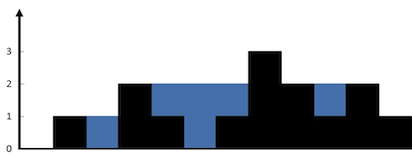
\includegraphics[width=7cm]{rain_water_trap}
    \label{fig:rain_water_trap}
\end{figure}

\paragraph{\color{white} \colorbox{OliveGreen}{Solution}}
\underline{$O(n)$ Time and $O(n)$ Space:}
$$W(i)=\min\{\max\{h_j|j\leqslant i\},\max\{h_k|k\geqslant i\}\}-h_i$$
where $W(i)$ denotes the largest water that the $i^{th}$ height can hold, $h_i$ denotes the $i^{th}$ height. We can modify the formula to
$$M_l(i)=\max\{h_j|j\leqslant i\}=\max\{M_l(i-1),i\}$$
$$M_r(i)=\max\{h_k|k\geqslant i\}=\max\{M_r(i+1),i\}$$
$$W(i)=\min\{M_l(i),M_r(i)\}-h_i$$
Using the method above, we have to scan the input and use extra space to record $M_l,M_r$, then we use $M_l,M_r$ to calculate each $W(i)$.


\underline{$O(n)$ Time and $O(1)$ Space:}
$$i_m=\arg_i\max h_i$$
\begin{equation*}
    W(i)=\begin{cases}
    \min\{M_l(i),h_{i_m}\}-h_i=M_l(i)-h_i & i\leqslant i_m\\
    \min\{h_{i_m},M_r(i)\}-h_i=M_r(i)-h_i & i>i_m
    \end{cases}
\end{equation*}
Using the method above, we scan the input to find the index of the highest height, $i_m$. Then, the $O(n)$ Space Method can be reduced to the $O(1)$ Space.

\subsection{150. Evaluate Reverse Polish Notation}

\paragraph{\color{white} \colorbox{Mahogany}{Description}}
Evaluate the value of an arithmetic expression in Reverse Polish Notation.

Valid operators are +, -, *, /. Each operand may be an integer or another expression.

\paragraph{\color{white} \colorbox{OliveGreen}{Solution}}
\underline{Code Hints}:
\begin{itemize}
    \item Stack is always related much to the problems such as recursion, expression evaluation, and parentheses evaluation.
\end{itemize}